\documentclass[11pt, a4paper]{MATH2023}
\usepackage{fancyhdr}
\usepackage{setspace}
\usepackage{amsmath,mathrsfs}
\usepackage{multicol}
\usepackage{amssymb}
\usepackage{graphicx}
\usepackage{caption}
\usepackage{subcaption}
\usepackage{xcolor}
\usepackage{enumitem}
\usepackage{tikz}
\usepackage{mathtools}
\usetikzlibrary{matrix}
\usepackage[normalem]{ulem}
\usepackage{multirow}
\usepackage[linesnumbered, ruled, boxed]{algorithm2e}
\SetKwRepeat{Do}{do}{while}
\newcommand{\eg}{\textbf{[Example.] }}
\newcommand{\sol}{\textbf{[Solution.] }}
\newcommand{\vct}{\underline}
\newcommand{\vv}{\underline{v}}
\newcommand{\uu}{\underline{u}}
\newcommand{\ww}{\underline{w}}
\newcommand{\rr}{\underline{r}}
\newcommand{\ii}{\underline{i}}
\newcommand{\kk}{\underline{k}}
\newcommand{\jj}{\underline{j}}
\newcommand{\va}{\underline{a}}
\newcommand{\bb}{\underline{b}}
\newcommand{\cc}{\underline{c}}
\newcommand{\dd}{\underline{d}}

\title{Chapter 10}
\subtitle{Vectors and Geometry in 3D}

\begin{document}
\begin{spacing}{1.3}
    \section{Coordinates in 3D}

    \eg $\{ (x,y,z)\mid z\ge \sqrt{x^2+y^2}\}$ is an ice-cream cone.

    \begin{center}
        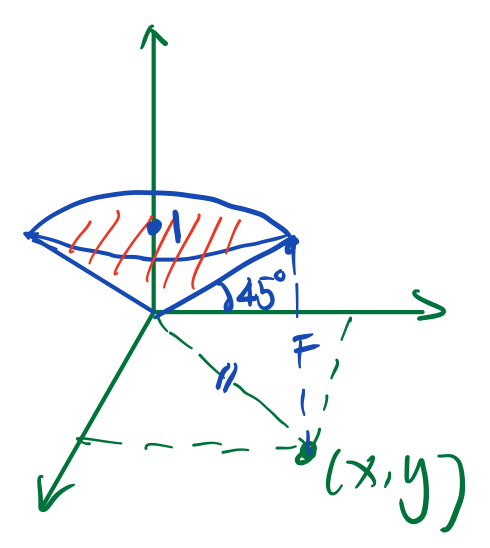
\includegraphics[scale=0.25]{images/Ch10-cone.jpeg}
    \end{center}
    {\bf Remark: }When one of the variables is missing from the equation, 
    the equation represents a surface {\it parallel} to the axis of the 
    missing variable.

    \eg $z=x^2$, since $y$ is missing, we draw a parabola and move it 
    along the $y$ axis.
    \begin{center}
        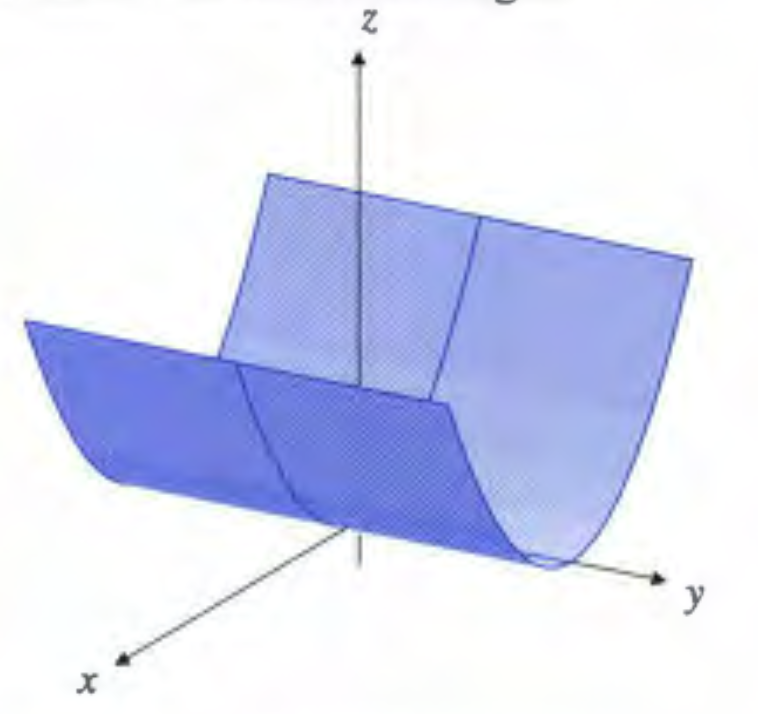
\includegraphics[scale=0.3]{images/Ch10-parabola-ymissing.png}
    \end{center}

    \section{Vectors}
    \subsection{Vectors and Properties}

    In $\mathbb{R}^3$, $\vct{r}=(a,b,c)=a\vct{i}+b\vct{j}+c\vct{k},\  
    ||\vct{r}||=\sqrt{a^2+b^2+c^2}$

    {\bf Zero vector} $\vct{0}$ has length zero and no specific direction.

    {\bf Properties of vectors}
    \begin{itemize}
        \item Equality: iff same {\bf magnitude }and same {\bf direction}.
        OR, their {\bf components} equal 
        \item Parallel: $\vct{r}=\lambda \vct{s}$
        \item Negative: $-\vct{r}$ has same magnitude but opposite direction.
        \item Addition, Subtraction, Scalar Multiplication: omit.
    \end{itemize}

    {\bf Unit Vector:} $\hat{\vct{r}}=\dfrac{\vct{r}}{||\vct{r}||}$

    {\bf Dot Product:} $\vct{u}\cdot \vct{v}=u_1v_1+u_2v_2+u_3v_3$.
    {\bf Remark: } $\vct{a}\cdot \vct{b}=\vct{a}\cdot \vct{c} \nRightarrow \vct{b}=\vct{c}$

    {\bf Angle:} $\vct{u}\cdot \vct{v}=||\vct{u}||\cdot ||\vct{v}||\cos\theta$

    {\bf Projections:}
    \begin{itemize}
        \item Scalar projection: $s=\dfrac{\vct{u}\cdot \vct{v}}{||\vct{v}||}=
        ||\vct{u}||\cos \theta$
        \item Vector projection of $\vct{u}$ in the direction of $\vct{v}$: 
        $\vct{u}_{\vct{v}}=\dfrac{\uu\cdot \vv}{||\vv||}\hat{\vv}=
        \dfrac{\uu\cdot \vv}{||\vv||^2}\vv$
    \end{itemize}

    \eg Find the scalar and vector projections of vector $\va=\ii-2\jj+\kk$ on
    the vector $\bb=4\ii-4\jj+7\kk$.

    \sol $$s=\frac{\va\cdot \bb}{||\bb||}=\frac{4+8+7}{\sqrt{4^2+4^2+7^2}}=\frac{19}{9}$$
    $$\va_{\bb}=s\cdot \frac{\bb}{||\bb||}=\frac{19}{81}(4\ii-4\jj+7\kk)$$

    {\bf Position Vector:} $\rr$ from the origin to the point $(a,b,c)$: 
    $$\rr = a\ii+b\jj+c\kk,\qquad ||\rr||=\sqrt{a^2+b^2+c^2}$$
    $$\hat{\rr}=\frac{a\ii+b\jj+c\kk}{\sqrt{a^2+B^2+c^2}}$$

    {\bf Cross Product:}
    \def\arraystretch{0.8}
    \begin{align*} 
        \uu \times \vv &=\left|
            \begin{array}{ccc}
                \ii & \jj & \kk \\ 
                u_{1} & u_{2} & u_{3} \\ 
                v_{1} & v_{2} & v_{3}
            \end{array}
            \right|
        =\left(u_{2} v_{3}-u_{3} v_{2}\right) \ii-
        \left(u_{1} v_{3}-u_{3} v_{1}\right) \jj+
        \left(u_{1} v_{2}-u_{2} v_{1}\right) \kk \\ 
        &=-\vv \times \uu \quad \text { \bf (vector) } 
    \end{align*}
    {\bf Properties:}
    \begin{itemize}
        \item $\uu\times \uu = \vct{0}$
        \item $\va\times(\bb+\cc)=\va\times \bb+\va\times \cc$
        \item $(\uu\times \vv)\cdot \uu=0, (\uu\times \vv)\cdot \vv=0$
        \item $||\uu\times \vv||=||\uu||\cdot ||\vv||\sin\theta=$ area of parallelogram.
        \begin{center}
            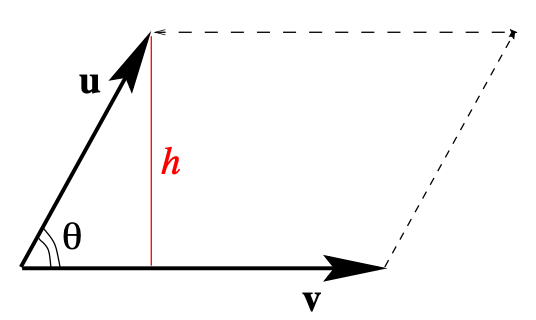
\includegraphics[scale=0.5]{images/Ch10-cross-product-geometry.png}
        \end{center}
        \item $||\uu \times \vv||^2=||\uu||^2||\vv||^2-(\uu\cdot \vv)^2$
        \item $\uu\times(\vv\times \ww)\ne (\uu\times \vv)\times \ww$
        \item $\vct{a}\times \vct{b}=\vct{a}\times \vct{c} \nRightarrow \vct{b}=\vct{c}$
    \end{itemize}

    \subsection{Triple Scalar Products}
    $$\va\cdot (\bb\times \cc)=a_{1}\left|
    \begin{array}
        {ll}b_{2} & b_{3} \\ 
        c_{2} & c_{3}
    \end{array}\right|-
    a_{2}\left|
    \begin{array}{ll}
        b_{1} & b_{3} \\ 
        c_{1} & c_{3}
    \end{array}\right|+
    a_{3}\left|
    \begin{array}{ll}
        b_{1} & b_{2} \\ 
        c_{1} & c_{2}
    \end{array}\right|=
    \left|
    \begin{array}{lll}
        a_{1} & a_{2} & a_{3} \\ 
        b_{1} & b_{2} & b_{3} \\ 
        c_{1} & c_{2} & c_{3}
    \end{array}\right|$$
    
    {\bf Geometric interpretation} of $\va\cdot (\bb\times \cc)$: 
    \begin{align*}
        \va\cdot (\bb\times \cc) &= ||\va||\ ||\bb\times \cc||\cos\theta \\
        &= \left(||\va||\cos\theta\right)\cdot ||\bb\times \cc||\\
        &= h\cdot ||\bb\times \cc||\\
        &= \textbf{volume of the parallelepiped}
    \end{align*}
    \begin{center}
        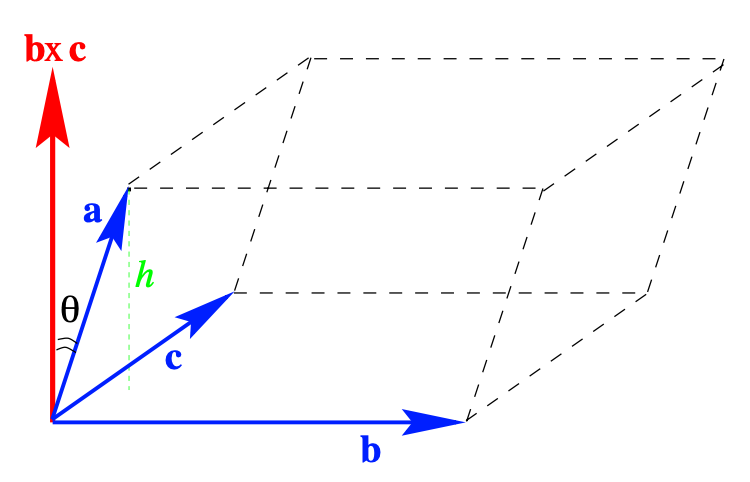
\includegraphics[scale=0.5]{images/Ch10-triple-scalar-prod.png}
    \end{center}

    Another use of triple scalar product is for deciding whether three 
    vectors are {\bf in the same plane}. If so, then $$(\va\times \bb)\cdot \cc=0$$

    \subsection{Triple Vector Products}

    $(\va\times \bb)\times \cc$ is in the plain containing $\va$ and $\bb$.
    \begin{center}
        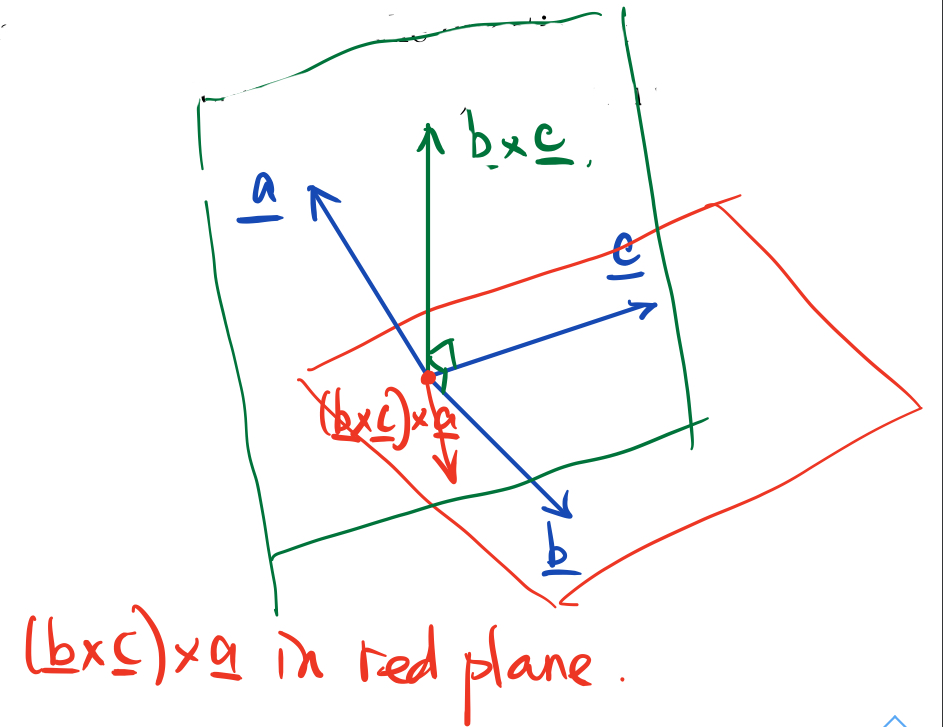
\includegraphics[scale=0.25]{images/Ch10-triple-cross-prod.jpeg}
    \end{center}

    \eg Construct three mutually orthogonal vectors in space, making use of 
    two non-parallel vectors $\va$ and $\bb$.

    \sol $\va$, $\va\times \bb$, and $\va\times(\va\times \bb)$.
    \begin{center}
        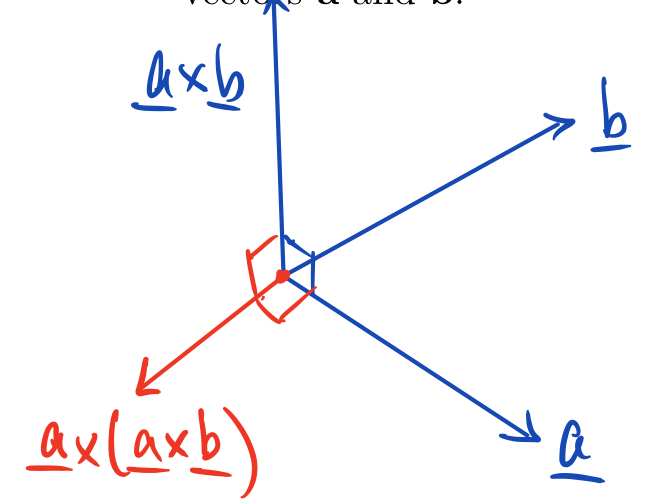
\includegraphics[scale=0.27]{images/Ch10-mutually-orth.jpeg}
    \end{center}

    \section{Planes and Lines}

    \subsection{Planes}

    {\bf The equation of a plane}: assume nonzero normal vector 
    $\vct{n}=A\ii+B\jj+C\kk$ and plane passes through $r_0=(x_0,y_0,z_0)$,
    $$\vct{n}\cdot (\vct{r}-\vct{r_0})=0$$
    can also written in {\bf standard form}: 
    $$Ax+By+Cz=Ax_0+By_0+Cz_0$$

    {\bf A pencil of planes}: a family of plans intersecting in a straight line.
    If two nonparallel planes have equations $A_1x+B_1y+C_1z=D1$ and 
    $A_2x+B_2y+C_2z=D_2$, then 
    $$A_1x+B_1y+C_1z-D1+\lambda(A_2x+B_2y+C_2z-D_2)=0$$
    represents a plane in the pencil, where $\lambda\in \mathbb{R}$.
    \begin{center}
        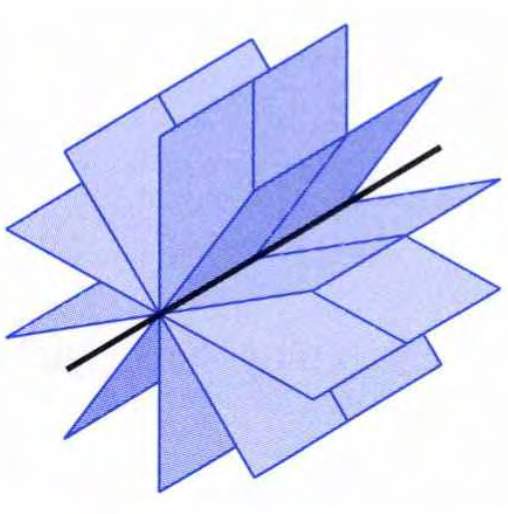
\includegraphics[scale=0.4]{images/Ch10-pencils-of-planes.png}
    \end{center}

    \eg Find the equation of the plane through $P_0=(-1,4,2)$ and 
    containing the line of intersection of the planes 
    $4x-y+z-2=0$ and $2x+y-2z-3=0$.

    \sol Two methods: 

    {\bf (1) find three points.} 

    Notice the two planes have infinity points intersected. 
    We arbitrarily choose 2 of them, say 
    $\vct{r_1}=(0,-7,-5), \vct{r_2}=(1,3,1)$. Another point is given in problem,
    $\vct{r_0}=(-1,4,2)$.

    Then a normal vector can be 
    $(\vct{r_1}-\vct{r_0})\times (\vct{r_2}-\vct{r_0})=(4,-13,21)$

    {\bf (2) find the pencil of planes.}

    The pencil of planes formed by the given two non-parallel planes is 
    $$4x-y+z-2+\lambda(2x+y-2z-3)=0$$
    Since the plane is inside the pencil and containing $P_0$,
    substitute $(-1,4,2)$ into the equation, we get $\lambda=-\dfrac{8}{5}.$

    \subsection{Lines}

    {\bf Vector parametric equation of straight line:} with a point 
    $\vct{r_0}$ and {\bf direction vector }$\vv$: 
    $$\vct{r}(t)=\vct{r_0}+t\vv$$

    \eg Find the vector equation for the line segment joins $P_1=(2,4,-1)$
    and $P_2=(5,0,7)$.

    \sol direction vector $\vv=(3,-4,8)$, thus 
    $$\vct{r}(t)=(2,4,-1)+t\cdot (3,-4,8),\ \red{0\le t\le 1}$$

    \eg Find the intersection of line $\vct{r}=\vct{r_0}+t\vct{v}$ 
    and plane $\vct{r}\cdot \vv=d$, assume they are not parallel.

    \sol $(\vct{r_0}+t\vv)\cdot \vct{n}=d$, solve for $t$.

    \subsection{Distances}

    {\bf Point to Line:} 

    \begin{center}
        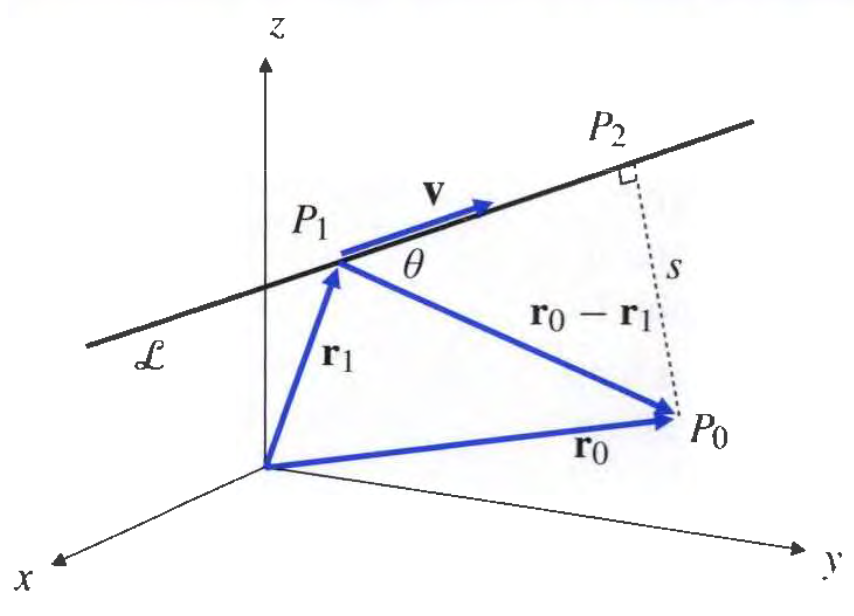
\includegraphics[scale=0.4]{images/Ch10-dist-point-line.png}
    \end{center}
    \begin{align*}
        d &= ||\vct{r_1}-\vct{r_0}||\cdot \sin\theta \cdot 1\\
         &= ||\vct{r_1}-\vct{r_0}||\cdot \sin\theta \cdot ||\hat{\vv}||\\
         &= ||(\vct{r_1}-\vct{r_0})\times \hat{\vv}||
    \end{align*}

    {\bf Point to Plane:} 
    \begin{align*}
        d &= ||\vct{r_1}-\vct{r_0}||\cdot \cos\theta \cdot 1\\
         &= ||\vct{r_1}-\vct{r_0}||\cdot \cos\theta \cdot ||\hat{\vct{n}}||\\
         &= | (\vct{r_1}-\vct{r_0})\cdot \hat{\vct{n}} |
    \end{align*}
    \begin{center}
        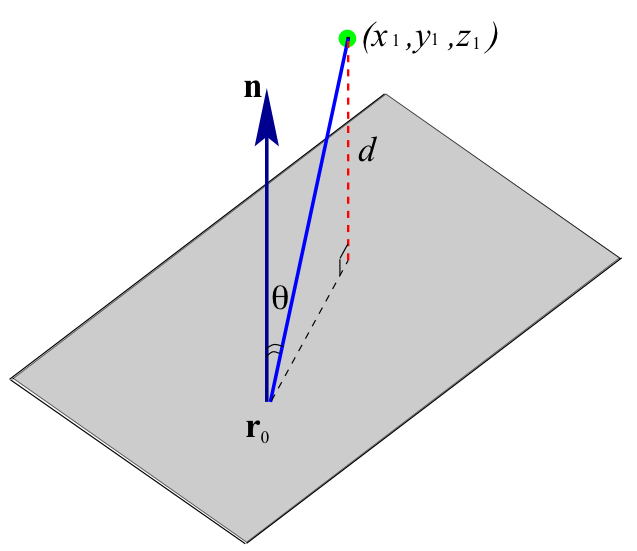
\includegraphics[scale=0.3]{images/Ch10-dist-point-plane-2.jpeg}
    \end{center}


    {\bf Line to Plane(parallel): } Take any point on the line $\rar$ point to plane.

    {\bf Parallel Lines: } Same as point to line.

    {\bf Skew Lines:} 

    \begin{center}
        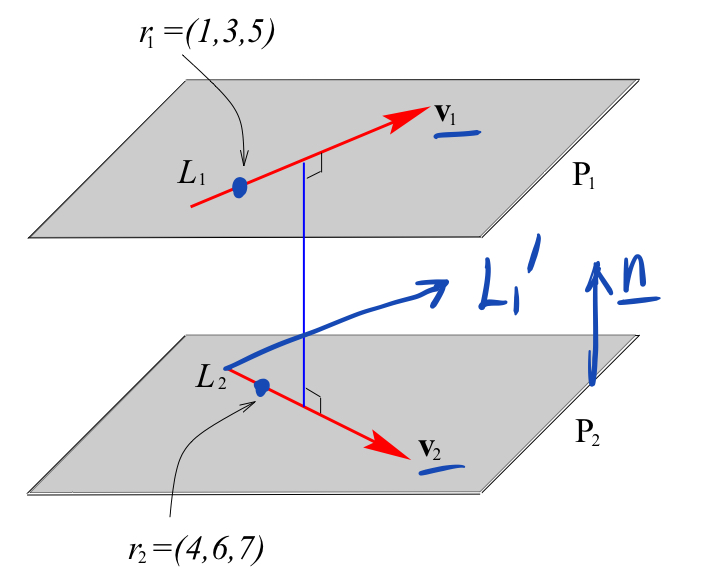
\includegraphics[scale=0.3]{images/Ch10-dist-line-line.jpeg}
    \end{center}

    Make $L_1$ and $L_1$ inside the same plane, then normal vector of 
    the plane is $\vct{n}=\vct{v_1}\times \vct{v_2}$.

    Now it is the same as line to plane.
    \begin{align*}
        d &= | (\vct{r_1}-\vct{r_0})\cdot \hat{\vct{n}} |\\
         &= | (\vct{r_1}-\vct{r_0})\cdot \widehat{(\vct{v_1}\times \vct{v_2})} |
    \end{align*}

    
    {\bf Plane to Plane(parallel):} same as point to plane. 


    \section{Quadric Surfaces}


    {\bf Spheres}: $(x-x_0)^2+(y-y_0)^2+(z-z_0)^2=a^2$.

    {\bf Cylinders:} $x^2+y^2=a^2$. (left below)

    {\bf Cones:} $z^2=x^2+y^2$. (right below)
    
    \begin{center}
        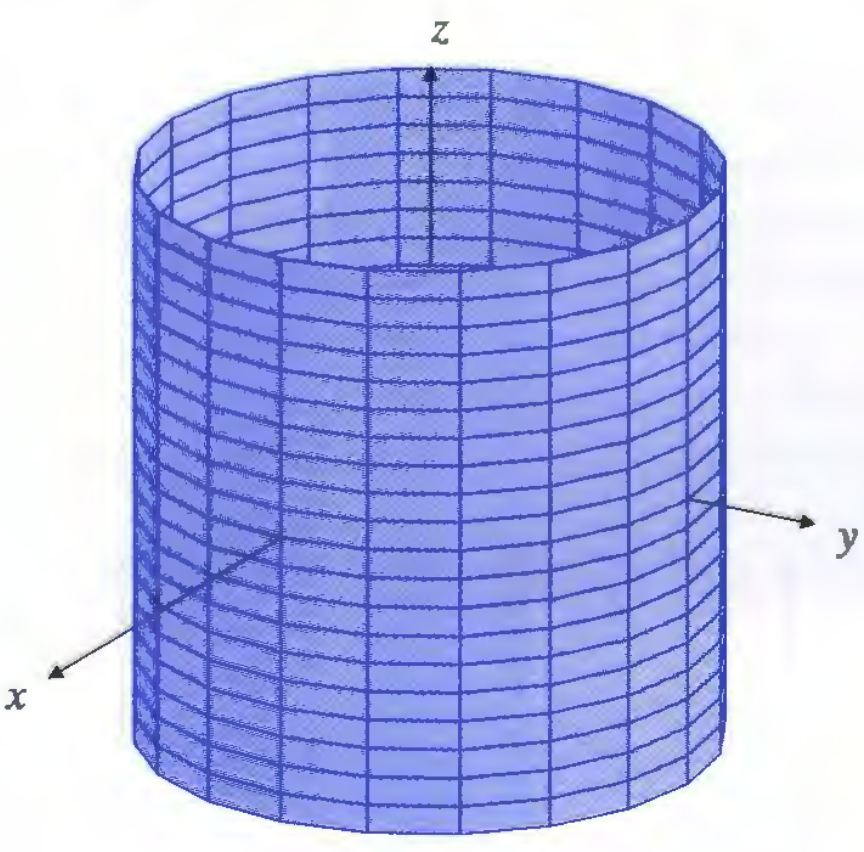
\includegraphics[scale=0.3]{images/Ch10-cylinder.png}
        \hspace{1in}
        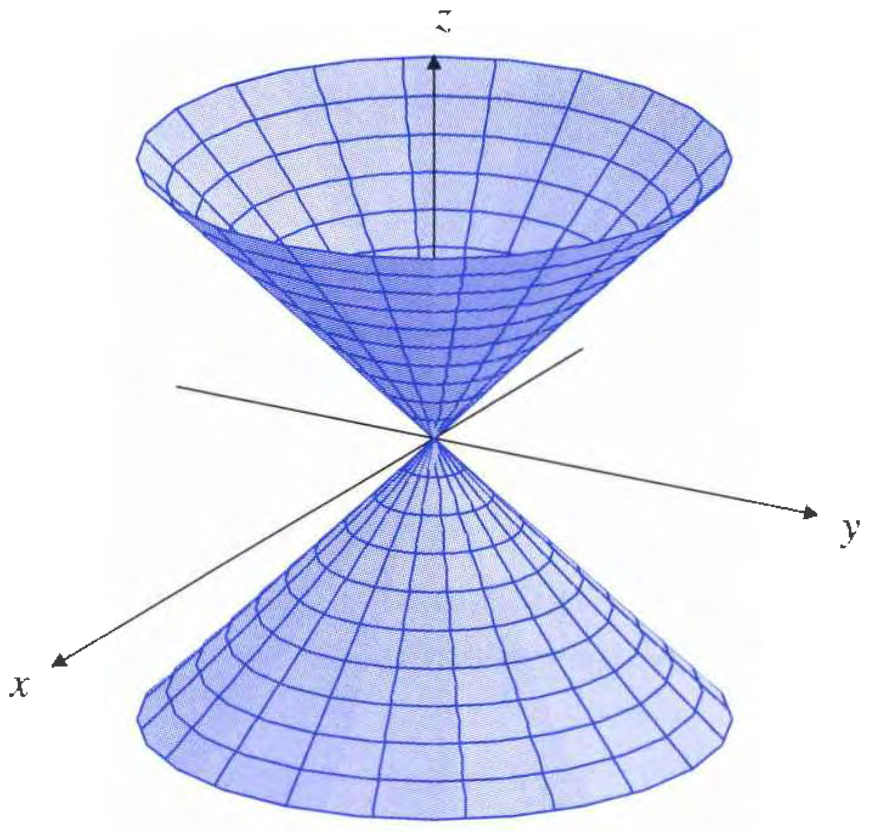
\includegraphics[scale=0.3]{images/Ch10-cone.png}
    \end{center}
    

    {\bf Ellipsoid:} $\disp \frac{x^2}{a^2}+\frac{y^2}{b^2}+\frac{z^2}{c^2}=1$. (left below)

    {\bf Elliptic paraboloid:} $\disp z=\frac{x^2}{a^2}+\frac{y^2}{b^2}$. (right below)

    \begin{center}
        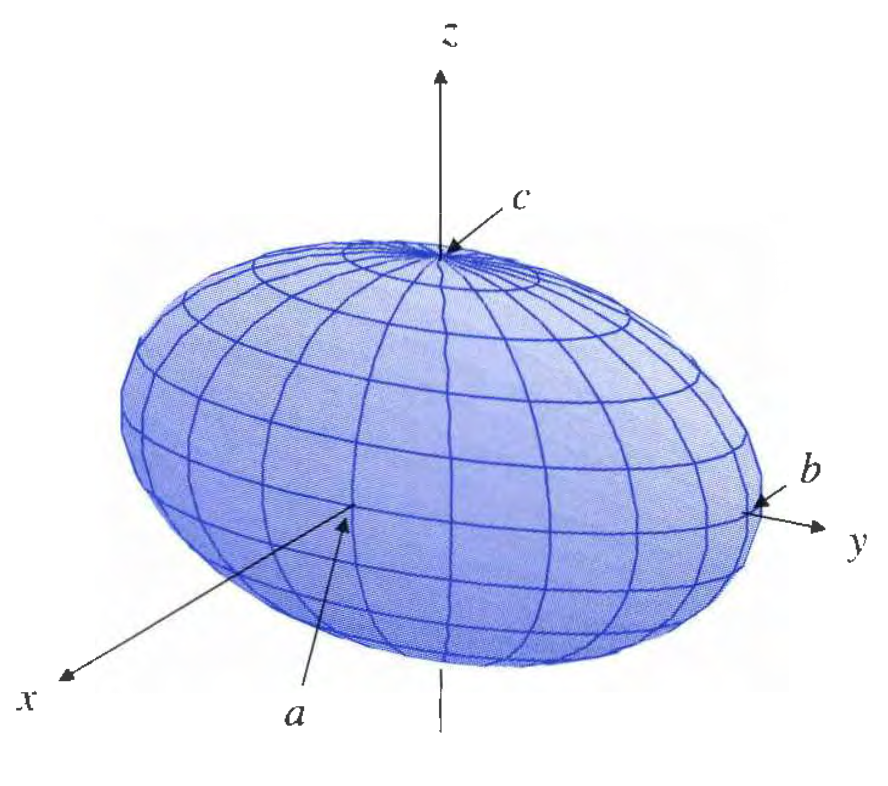
\includegraphics[scale=0.3]{images/Ch10-ellipsoid.png}
        \hspace{1in}
        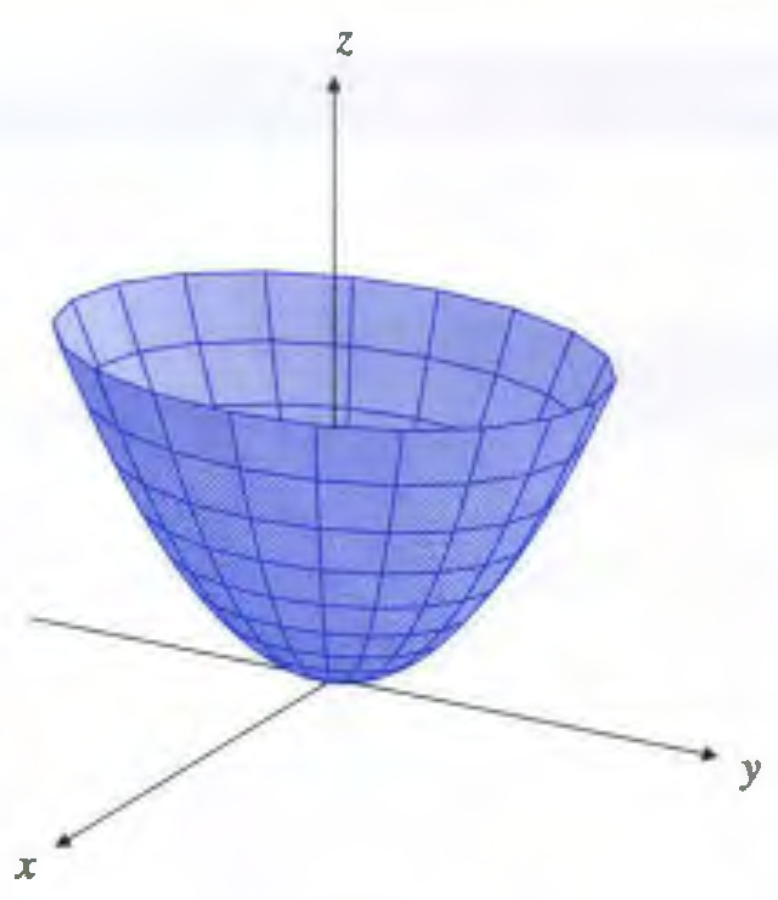
\includegraphics[scale=0.3]{images/Ch10-elliptic-paraboloid.png}
    \end{center}

    {\bf Hyperbolic paraboloid :} $\disp z=\frac{x^2}{a^2}-\frac{y^2}{b^2}$.

    \begin{center}
        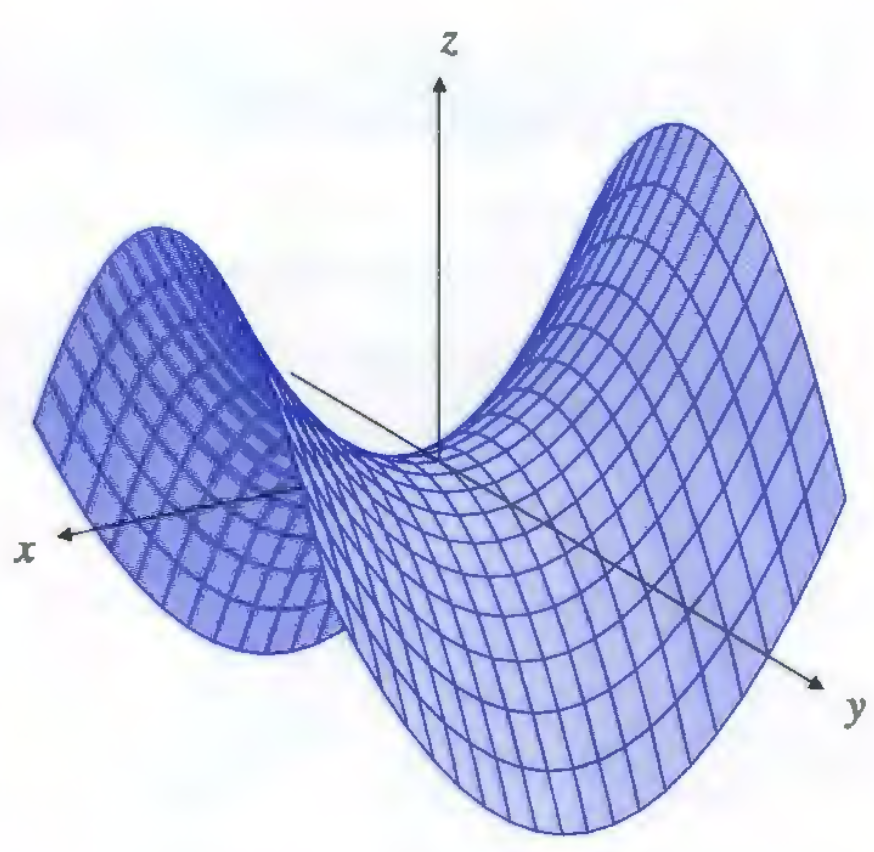
\includegraphics[scale=0.3]{images/Ch10-hyperbolic-paraboloid.png}
    \end{center}

    {\bf Hyperboloids:}
    \begin{center}
        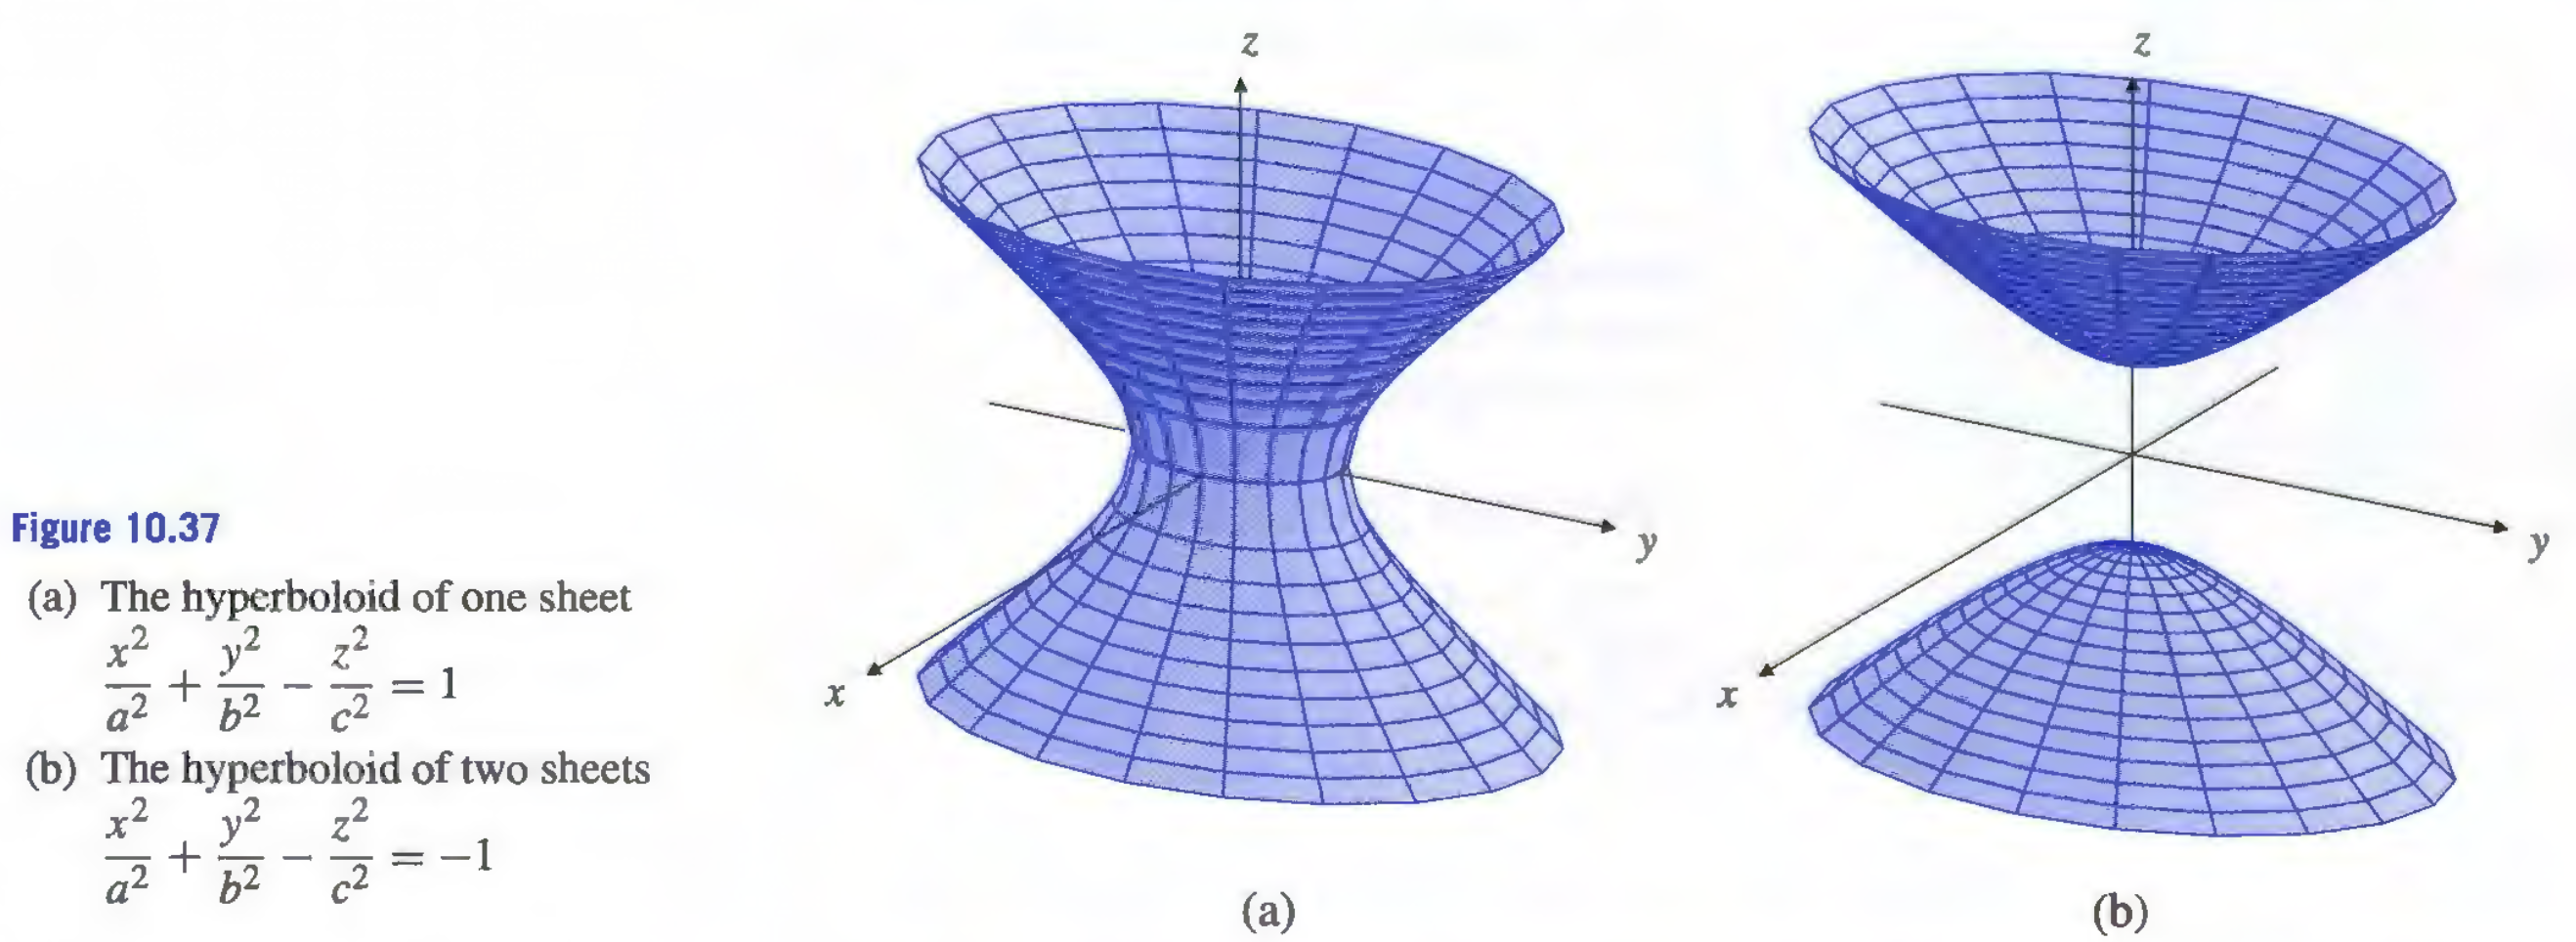
\includegraphics[scale=0.37]{images/Ch10-hyperboloid.png}
    \end{center}

    \section{Cylindrical and Spherical Coordinates}

    {\bf Cylindrical Coordinate:} $(r,\theta,z)$
    \begin{align*}
        x &= r\cos\theta\\ y&=r\sin\theta\\z&=z
    \end{align*}
    where $r\ge 0,\ 0\le \theta<2\pi$, and 
    \begin{align*}
        r &= \sqrt{x^2+y^2}\\
        \theta &= \left\{ \begin{array}{ll}
            \tan^{-1}(y/x) & {\rm if}\ x\ge 0\\
            \tan^{-1}(y/x)+\pi & {\rm if}\ x<0
        \end{array}\right.
    \end{align*}

    \begin{center}
        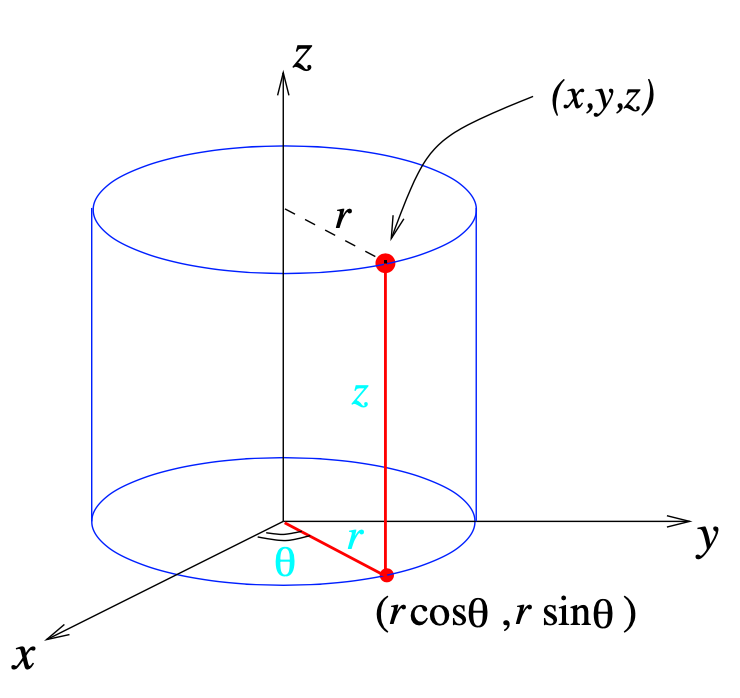
\includegraphics[scale=0.4]{images/Ch10-cylindrical-coor.png}
        \hspace{1in}
        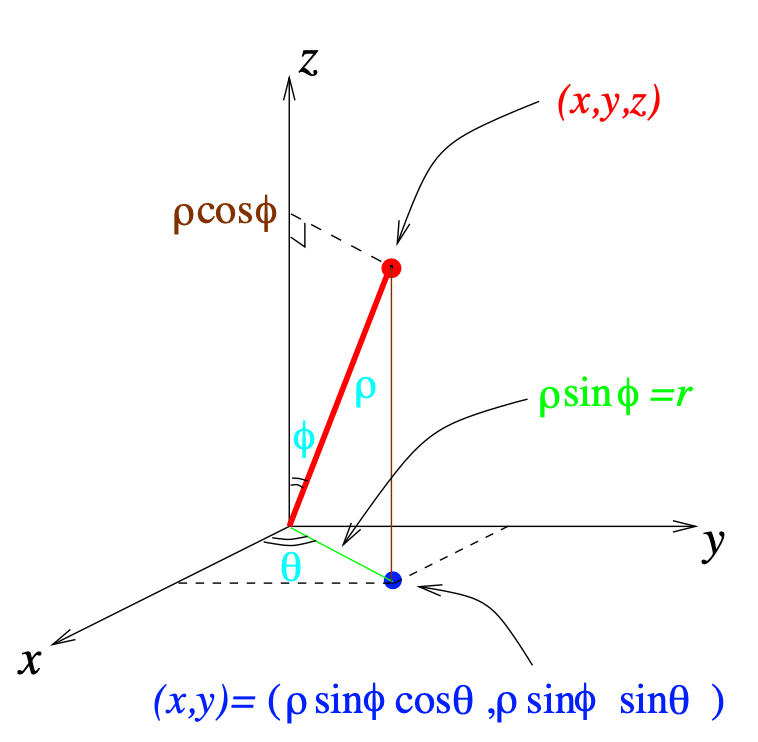
\includegraphics[scale=0.4]{images/Ch10-spherical-coor.png}
    \end{center}

    {\bf Spherical Coordinates: } $(\rho, \theta,\phi)$
    \begin{align*}
        x &= r\cos\theta=\rho\sin\phi\cos\theta\\
        y &= r\sin\theta=\rho\sin\phi\sin\theta\\
        z &= \rho\cos\phi
    \end{align*}
    where $\rho\ge 0,\ 0\le \theta<2\pi,\ 0\le \phi\le \pi$, and 
    \begin{align*}
        \rho &= \sqrt{x^2+y^2+z^2}\\
        \theta &= \left\{ \begin{array}{ll}
            \tan^{-1}(y/x) & {\rm if}\ x\ge 0\\
            \tan^{-1}(y/x)+\pi & {\rm if}\ x<0
        \end{array}\right.\\
        \phi &= \cos^{-1}(z/\rho)
    \end{align*}


\end{spacing}
\end{document}
